\documentclass{article}
\usepackage[utf8]{inputenc}
\usepackage{amsmath}
\usepackage{geometry}
\geometry{
 a4paper,
 total={182mm,257mm},
 left=14mm,
 top=20mm,
 }
 \usepackage{amsthm}
 \usepackage[utf8]{inputenc}
 \usepackage[italian]{babel}
\usepackage[T1]{fontenc}
\usepackage{amssymb}
\usepackage{physics}
\usepackage{commath}
\usepackage{tikz}
\usepackage{pgfplots}
\usepackage{graphicx}
\graphicspath{ {Immagini/} }
\usepackage{float}
\usepackage{hyperref}
\hypersetup{
    colorlinks=true,
    linkcolor=red,
    citecolor=green
    filecolor=magenta,      
    urlcolor=cyan,
}


%Theorem Environments
\newtheorem{thm}{Teorema}[section]
\newtheorem{lem}[thm]{Lemma}
\newtheorem{property}{Proprietà}[section]
\newtheorem{defn}{Definizione}[section]
\newtheorem{prop}[defn]{Proposizione}
\newtheorem{example}{Esempi}[subsection]
\newtheorem{exerc}[example]{Esercizi Svolti}

%Commandi di Formattazione
\newcommand{\noi}{\noindent}
\newcommand{\note}{\noindent {\quad \bf \underline{Osservazione:}} \quad}
\newcommand{\eg}{\noindent {\bf \underline{Esempio:}} \quad}
\newcommand{\bfemph}[1]{\textbf{\textit{#1}}}
\renewcommand{\emph}[1]{\bfemph{#1}}

%Number Sets
\newcommand{\R}{\mathbb{R}}
\newcommand{\C}{\mathbb{C}}
\newcommand{\Z}{\mathbb{Z}}
\newcommand{\Q}{\mathbb{Q}}

%Shortcuts
\newcommand{\then}{\ensuremath{\Rightarrow}}
\newcommand{\twopartdef}[4]
{
	\left\{
		\begin{array}{ll}
			#1 & \mbox{se } #2 \\
			#3 & \mbox{se } #4
		\end{array}
	\right.
}

%Vectors
\renewcommand{\i}{\vu{i}}
\renewcommand{\j}{\vu{j}}
\renewcommand{\k}{\vu{k}}
\renewcommand{\a}{\va{a}}
\renewcommand{\b}{\va{b}}
\renewcommand{\c}{\va{c}}
\renewcommand{\v}{\va{v}}
\renewcommand{\u}{\va{u}}
\newcommand{\s}{\va{s}}
\renewcommand{\t}{\va{t}}
\newcommand{\verst}{\vu{t}}
\newcommand{\versr}{\vu{r}}
\renewcommand{\r}{\va{r}}
\newcommand{\tauvs}{\vu{\tau}}
\newcommand{\tauvt}{\va{\tau}}
\newcommand{\normvs}{\vu{n}}
\newcommand{\N}{\va{N}}
\newcommand{\g}{\va{g}}
\newcommand{\F}{\va{F}}
\newcommand{\f}{\va{f}}
\newcommand{\M}{\va{M}}
\renewcommand{\l}{\va{l}}
\newcommand{\p}{\va{p}}
\renewcommand{\P}{\va{P}}
\renewcommand{\L}{\va{L}}


\renewcommand{\c}{\overline{c}}
\title{Il Primo Principio della Termodinamica}
\author{Roberto Gargiulo}
\date{Ultimo Aggiornamento: \today}


\begin{document}

\maketitle
\tableofcontents

\paragraph{Trasformazioni Termodinamiche}
Parliamo di \textbf{trasformazione termodinamica} da uno stato iniziale ad uno stato finale un passaggio da un'equilibrio termodinamico ad un altro. In generale tale trasformazione risulta impossibile da rappresentare su un piano termodinamico p-V in quanto solo agli equilibri le grandezze termodinamiche sono ben definite. Possiamo però rappresentare come segue una trasformazione di questo tipo:
\begin{figure}[H]
    \centering
    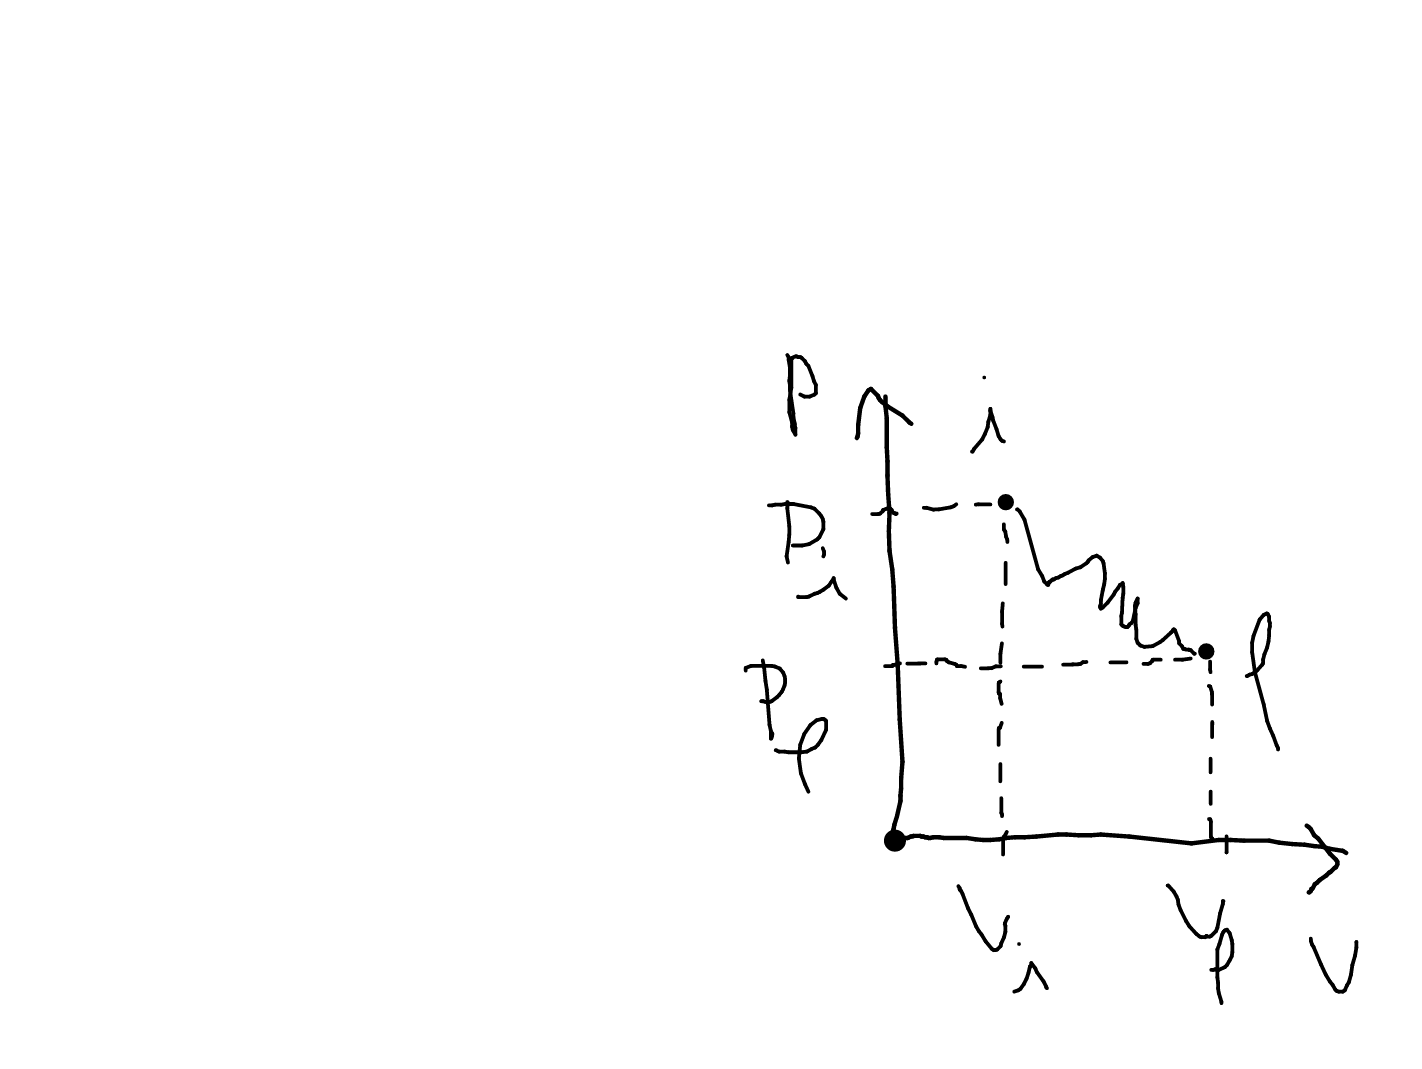
\includegraphics[width=0.5\textwidth]{TrasformazioneIrreversibile.png}
    \caption{Esempio di Trasformazione Termodinamica}
    \label{TrasfIrrev}
\end{figure}

Possiamo quindi formulare il \textbf{Primo Principio della Termodinamica} come segue: la variazione di \textbf{energia interna} è la differenza tra il calore scambiato con l'esterno e il lavoro compiuto (o subito) dal sistema.
\begin{equation}
    \boxed{Q-L=\Delta U}
\end{equation}
\paragraph{Trasformazioni Infinitesime}
Queste sono trasformazioni ottenute per infinitesime quantità di calore e lavoro scambiati con l'esterno da un sistema (a cui corrispondono infinitesima variazioni di pressione, volume e temperatura). Studiando un sistema con varianza 2 otteniamo il primo principio per quantità infinitesima:
\[\delta Q-\delta L=\dif U\]
Notiamo che Q ed L sono forme differenziali in quanto non sono funzioni di stato, diversamente dall'energia interna. Calcoliamo la quantità di calore infinitesima fornita utilizzando la definizione di lavoro e la proprietà di differenziale esatto di energia interna:
\[\delta Q=\dif U+\delta L=\left(\pdv{U}{t}\right)_V\dif t+\left(\pdv{U}{V}\right)_t\dif V+p^{(e)}\dif V\]
Otteniamo quindi la seguente \textbf{formula del calore} per trasformazioni infinitesime:
\begin{equation}
\boxed{\delta Q=\left(\pdv{U}{t}\right)_V\dif t+\left[\left(\pdv{U}{V}\right)_t+p^{(e)}\right]\dif V}
\end{equation}
Per una trasformazione infinitesima \textbf{isocora} si riduce a:
\[\delta Q=\left(\pdv{U}{t}\right)_V\dif t\]
Ma per definizione di calore specifico molare:
\[\dv{Q}{t}=\left(\pdv{U}{t}\right)_V=n\overline{c}_V\then \boxed{\delta Q=n\overline{c}_V\dif t+\left[\left(\pdv{U}{V}\right)_t+p^{(e)}\right]\dif V}\]
Siccome l'energia interna è una funzione di stato, questa espressione è valida per ogni trasformazione infinitesima.
Per i liquidi e i solidi, considerati incompressibili possiamo porre $\dif V=0$, mentre il calore specifico molare è uguale sia a pressione che a volume costante. Pertanto il calore si riduce all'espressione della trasformazione isocora per liquidi e solidi.

\section{I Gasi Ideali}
Per quanto riguarda i gas, il comportamento si può generalizzare ad ogni gas nel caso in cui essi siano \textbf{rarefatti}, ossia poco densi e ad alta temperatura. In particolare valgono le seguenti leggi:
\begin{enumerate}
    \item La Prima Legge di Gay-Lussac \[V=V_0(1+\alpha t)\]
    Dove $\alpha$ è una costante che vale $\frac{1}{273,16^\circ C}$ per gas rarefatti, $V_0$ è il volume a pressione atmosferica e $0^\circ C$ e la pressione è costante.
    \item La Seconda Legge di Gay-Lussac \[p=p_0(1+\alpha t)\]
    Con volume costante e dove $p_0$ è la costante atmosferica.
    \item La Legge di Boyle \[pV=p_0V_0\]
    Che è valida a temperatura costante.
\end{enumerate}
Da queste leggi possiamo ricavare l'\textbf{equazione di stato} per i gas ideali. Immaginiamo di sottoporre il gas ad una trasformazione isobara, vale allora la prima legge di Gay-Lussac:
\[V_1=V_0(1+\alpha t)\]
Sottoponiamola poi ad una trasformazione isoterma, in modo che sia valida la legge di Boyle:
\[pV=p_0V_1=p_0V_0(1+\alpha t)\]
Esplicitando $V_0$ come prodotto del numero di moli e del volume molare otteniamo (abbiamo implicitamente usato la \textbf{Legge di Avogadro} nell'affermare che tutti i gas rarefatti hanno lo stesso volume molare):
\[pV=p_0n\overline{v}_0\alpha \left(t+\frac{1}{\alpha}\right)\]
Definiamo quindi una nuova scala di temperatura, detta \textbf{scala di Kelvin} tale che $\theta=(t+273,16)K$ e poi definiamo la \textbf{costante universale dei gas} come $R=p_0\overline{v}_0\alpha$ ottenendo infine:
\begin{equation}
\boxed{pV=nR\theta}
\end{equation}
Ossia l'equazione di stato dei gas perfetti.

\section{Il II Esperimento di Joule}
\begin{figure}[H]
    \centering
    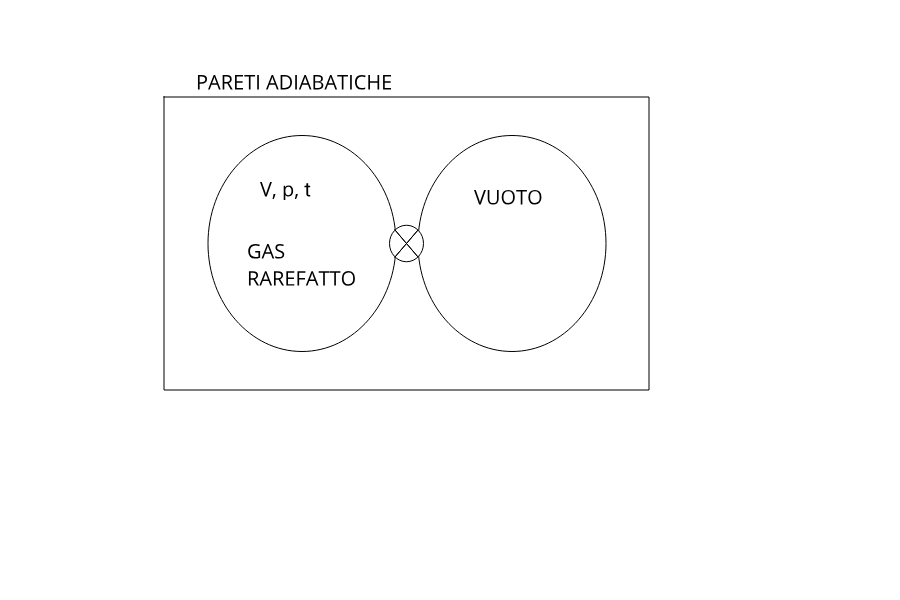
\includegraphics[width=0.5\textwidth]{SecondoJoule.png}
    \caption{Stato Iniziale del Secondo Esperimento di Joule}
    \label{SecondoJoule}
\end{figure}
Costruiamo un sistema isolato con delle pareti adiabatiche dall'esterno e in contatto con un altro contenitore tramite una valvola. Immaginiamo di \textbf{bruscamente} aprire questa valvola, otterremo che all'equilibrio il gas occupa tutto il volume. Inoltre si può misurare che all'equilibrio la temperatura risulta invariata:\\
\begin{center}
\begin{tabular}{c|c|c|c}
    INIZIO & $V_i=V_1$ & $p_i=p_0$ & $t_i=t_1$ \\
    \hline
    FINE & $V_f=V_1+V_2$ & // & $t_f=t_1$
\end{tabular} 
\end{center}
Ripetendo l'esperimento a densità molare decrescente otteniamo il seguente grafico:\\
\begin{center}
\begin{tikzpicture}
\begin{axis}[
    axis lines = left,
    xlabel = $\frac{n}{V_i}$,
    ylabel = {$t_i-t_f$},
]
\addplot [
    domain=0:10, 
    samples=10, 
    color=red,
]
{x*0.3};
\end{axis}
\end{tikzpicture}
\end{center}
Ossia otteniamo una funzione che tende a 0 al calare della densità molare. Osserviamo inoltre che essendo le pareti adiabatiche e fisse, esse isolano il sistema sia meccanicamente che termicamente in modo che non ci siano scambi di calore nè l'ambiente possa compiere lavoro sul sistema (o viceversa), quindi la variazione di energia interna è nulla:
\[\Delta U=Q-L=0\then U_i=U_f\]
Scelte t e V come variabili termodinamiche del sistema allora vale:
\[U(t_1,V_1)=U(t_1,V_1+V_2)=U(t_1,yV_1)\]
Ossia il volume a temperatura costante varia linearmente, quindi:
\[\pdv{U}{V}=0\then U=U(t)=U(\theta)\]
Ossia l'energia interna è una \textbf{funzione di stato} che dipende unicamente dalla \textit{temperatura}.\\
Pertanto un gas ideale è descritto termodinamicamente dall'equazione di stato e della funzione energia interna:
\begin{equation}
\begin{cases}
pV=nR\theta\\
U=U(\theta)
\end{cases}
\end{equation}
Per un gas ideale vale allora la seguente espressione di calore ed energia interna:
\begin{equation}
\boxed{(\delta Q)_V=n\overline{c}_V\dif\theta=\dif U}\then \boxed{U(\theta)=\int n\overline{c}_V(\theta)\dif\theta+cost}
\end{equation}
Queste considerazioni (fatte in questa situazione) sono tuttavia valide in ogni trasformazione termodinamica, in quanto l'energia interna è una funzione di stato. Mentre l'espressione generale del calore è:
\[\delta Q=n\overline{c}_V\dif\theta+p^{(e)}\dif V\]
\paragraph{Calore Specifico Molare}
Il calore specifico molare a volume costante per i gas si comporta (sommariamente) come in figura, dove i monoatomici hanno $\overline{c}_V$ costante, i biatomici hanno $\overline{c}_V$ a "scaletti" a cui corrisponde microscopicamente lo "sblocco" dei gradi di libertà delle molecole e infini i poliatomici hanno andamenti altamente complicati, la cui curva tende a diventare più \textit{liscia} all'aumentare degli atomi componenti. Generalmente la fascia considerata è quella in cui i gas biatomici hanno $\overline{c}_V=\frac{5}{2}R$ e i monoatomici hanno $\overline{c}_V=\frac{3}{2}R$.\\
Vale inoltre la \textbf{legge di Mayer} che stabilisce che:
\begin{equation}
\boxed{\overline{c}_p-\overline{c}_V=R}
\end{equation}

\subsection{Trasformazioni Reversibili}
\begin{defn}[Trasformazione Quasistatica]
Si definisce trasformazione \textbf{quasistatica} una trasformazione ottenuta tramite somma di trasformazioni infinitesime. Praticamente ciò implica che una trasformazione quasistatica si può rappresentare sul piano p-V:
\[\int_A^B\delta Q-\int_A^B\delta L=\int_A^B\dif U\]
In questo caso sono ben definite tutte le grandezze termodinamiche per ogni variazione allora per il calcolo del lavoro possiamo utilizzare la pressione del gas (uguale a quella esterna). 
\end{defn}
\begin{defn}[Trasformazione Reversibile]
Una trasformazione quasistatica si dice reversibile se può essere ripetuta in senso inverso seguendo gli stessi stati di equilibrio punto per punto. 
\end{defn}
Tra le più comuni trasformazioni reversibili individuiamo le seguenti quattro:
\begin{figure}[H]
    \centering
    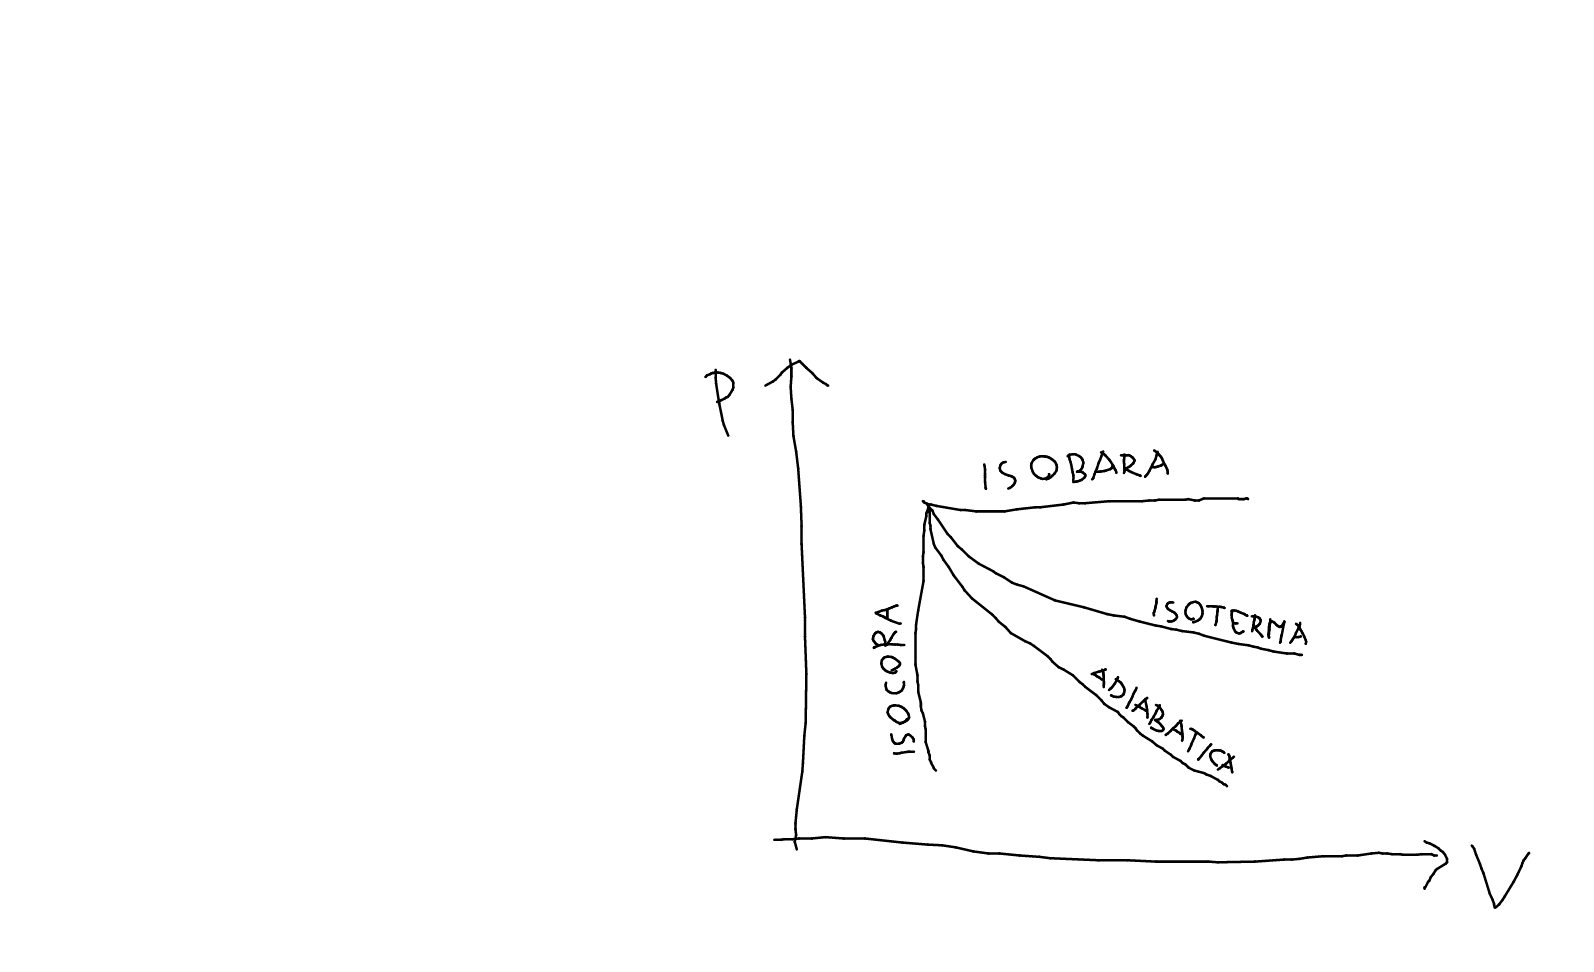
\includegraphics[width=0.6\textwidth]{TrasformazioniReversibili.png}
    \caption{Le Maggiori Trasformazioni Reversibili }
    \label{TrasfRevers}
\end{figure}
\paragraph{Trasformazione Adiabatica Reversibile} Considerando un'adiabatica reversibile possiamo applicare il primo principio per le trasformazioni infinitesime e poi integrando tra uno stato A e B:
\[\delta Q=\dif U+\delta L=n\overline{c}_V\dif\theta+p\dif V=0\then \overline{c}_V\frac{\dif\theta}{\theta}+R\frac{\dif V}{V}=0\then \overline{c}_V\ln\frac{\theta_B}{\theta_A}+R\ln\frac{V_B}{V_A}=0\]
Definita la costante $\gamma=\frac{\overline{c}_p}{\overline{c}_V}$ allora possiamo esplicitare come segue:
\begin{equation}
\begin{split}
    \ln\frac{\theta_B}{\theta_A}+\frac{R}{\overline{c}_V}\ln\frac{V_B}{V_A}&=0\\
    \ln\frac{\theta_B}{\theta_A}+(\gamma-1)\ln\frac{V_B}{V_A}&=0\\
    \ln\frac{\theta_B}{\theta_A}+\ln\left(\frac{V_B}{V_A}\right)^{\gamma-1}&=0\\
    \ln\left[\frac{\theta_B}{\theta_A}\left(\frac{V_B}{V_A}\right)^{\gamma-1}\right]&=0\\
\end{split}
\end{equation}
Per le proprietà dei logaritmi otteniamo:
\[\frac{\theta_B}{\theta_A}\left(\frac{V_B}{V_A}\right)^{\gamma-1}=1\then \theta_BV_B^{\gamma-1}=\theta_AV_A^{\gamma-1}\]
Ossia:
\begin{equation}
\boxed{\theta V^{\gamma-1}=cost}
\end{equation}
Utilizzando l'equazione di stato dei gas ideali possiamo anche ottenere le seguenti espressioni:
\[pV^{\gamma}=cost\quad Tp^{\frac{1-\gamma}{\gamma}}\]

\end{document}